\documentclass[conference]{IEEEtran}

\usepackage{graphicx}
\usepackage{booktabs}
\usepackage{amsmath,amssymb}
\usepackage{cite}
\usepackage{url}

\title{AI-Powered Skin Lesion Classification for Melanoma Detection (DSCI 498)}

\author{\IEEEauthorblockN{Yue Yu}}

\begin{document}
\maketitle

\begin{abstract}
This paper presents an end-to-end deep learning system for dermatoscopic skin lesion classification on HAM10000, a seven-class benchmark with strong class imbalance and clinically important melanoma cases. The goal is not only to obtain strong overall multiclass accuracy, but also to analyze how training choices and decision thresholds affect melanoma sensitivity. I compare EfficientNet-based classifiers with class-weighted loss, weighted sampling, melanoma upweighting, synthetic augmentation, and threshold-based melanoma screening. On a fixed lesion-wise split, the best accuracy-focused model, EfficientNet-B2 at 260px, achieves 0.8614 test accuracy and 0.7386 macro-F1, while a sensitivity-first training setup reaches 0.8548 top-1 melanoma recall at the cost of much lower overall accuracy. I further extend the evaluation with post-hoc confidence calibration and subgroup analysis using HAM10000 metadata. The accuracy-focused model shows mild overconfidence with mean top-1 confidence 0.8735 versus 0.8614 accuracy and expected calibration error 0.0484. The main conclusion is that the ``best'' model depends on whether the target is multiclass prediction, melanoma-sensitive screening, or reliable confidence estimates.
\end{abstract}

\section{Introduction}
Skin lesion classification is a high-impact computer vision task because early melanoma detection can reduce diagnostic delay, yet false negatives can be costly. Deep neural networks have shown strong performance on curated dermatology benchmarks \cite{esteva2017dermatologist}, but medical imaging systems remain vulnerable to class imbalance, limited external validation, and overconfident probability estimates \cite{tschandl2018ham10000,melo2025systematic}. These issues are especially important for HAM10000, where benign nevi dominate the dataset and can inflate accuracy while hiding clinically relevant errors.

This project studies an end-to-end classifier for HAM10000 with three linked goals: 1) strong multiclass performance, 2) explicit melanoma sensitivity analysis, and 3) confidence and subgroup diagnostics beyond headline accuracy. The central claim is that a single training objective does not capture the real operating trade-off: the strongest accuracy-focused model is not the strongest melanoma detector, and a sensitivity-first operating mode improves melanoma recall at a substantial cost in overall utility.

The contribution is practical rather than architectural. I build a reproducible EfficientNet-based pipeline, compare several imbalance-handling strategies, analyze threshold-based melanoma screening, and add post-hoc confidence calibration plus metadata-based subgroup analysis. This makes the final system more complete and more realistic as a medical-AI style course project.

\section{Related Work}
CNN-based skin lesion classification has been studied extensively, with landmark work showing dermatologist-level performance on curated datasets \cite{esteva2017dermatologist}. More recent surveys emphasize that apparent performance gains can still hide important weaknesses in class imbalance handling, robustness, subgroup behavior, and reporting quality \cite{khan2021survey,melo2025systematic}. HAM10000 has become a widely used benchmark precisely because it exposes some of these issues: it is clinically relevant, multi-source, and strongly imbalanced \cite{tschandl2018ham10000}.

This project is positioned closer to an evaluation-driven medical AI pipeline than to a novel architecture paper. The main distinction is that it does not stop at reporting a best accuracy number. Instead, it explicitly compares overall multiclass accuracy, melanoma-sensitive operating modes, and post-hoc reliability diagnostics inside one reproducible framework. It also connects to prior work that uses class-rebalancing losses \cite{cui2019classbalanced} or patient clinical information \cite{elngar2022clinicalinfo}, but keeps the final system lightweight enough for a course project.

\section{Dataset and Task}
HAM10000 contains 10{,}015 dermatoscopic images with seven diagnostic categories and associated metadata such as lesion ID, age, sex, and anatomical localization \cite{tschandl2018ham10000}. The target classes are \texttt{akiec}, \texttt{bcc}, \texttt{bkl}, \texttt{df}, \texttt{mel}, \texttt{nv}, and \texttt{vasc}. The dataset is severely imbalanced: \texttt{nv} contributes about 67\% of all samples, while several categories are below 5\%.

To avoid leakage, I use a lesion-wise grouped split based on \texttt{lesion\_id}, producing 8012 train images, 1000 validation images, and 1003 test images. This prevents multiple images from the same lesion from appearing in both train and test.

HAM10000 also contains metadata fields such as diagnosis type, sex, age, and localization. These attributes are useful for understanding possible sources of bias and heterogeneity even when the classifier itself is image-only. In particular, the dataset mixes multiple acquisition sources and multiple forms of diagnostic confirmation, which makes it a realistic but imperfect medical benchmark.

\begin{figure}[t]
  \centering
  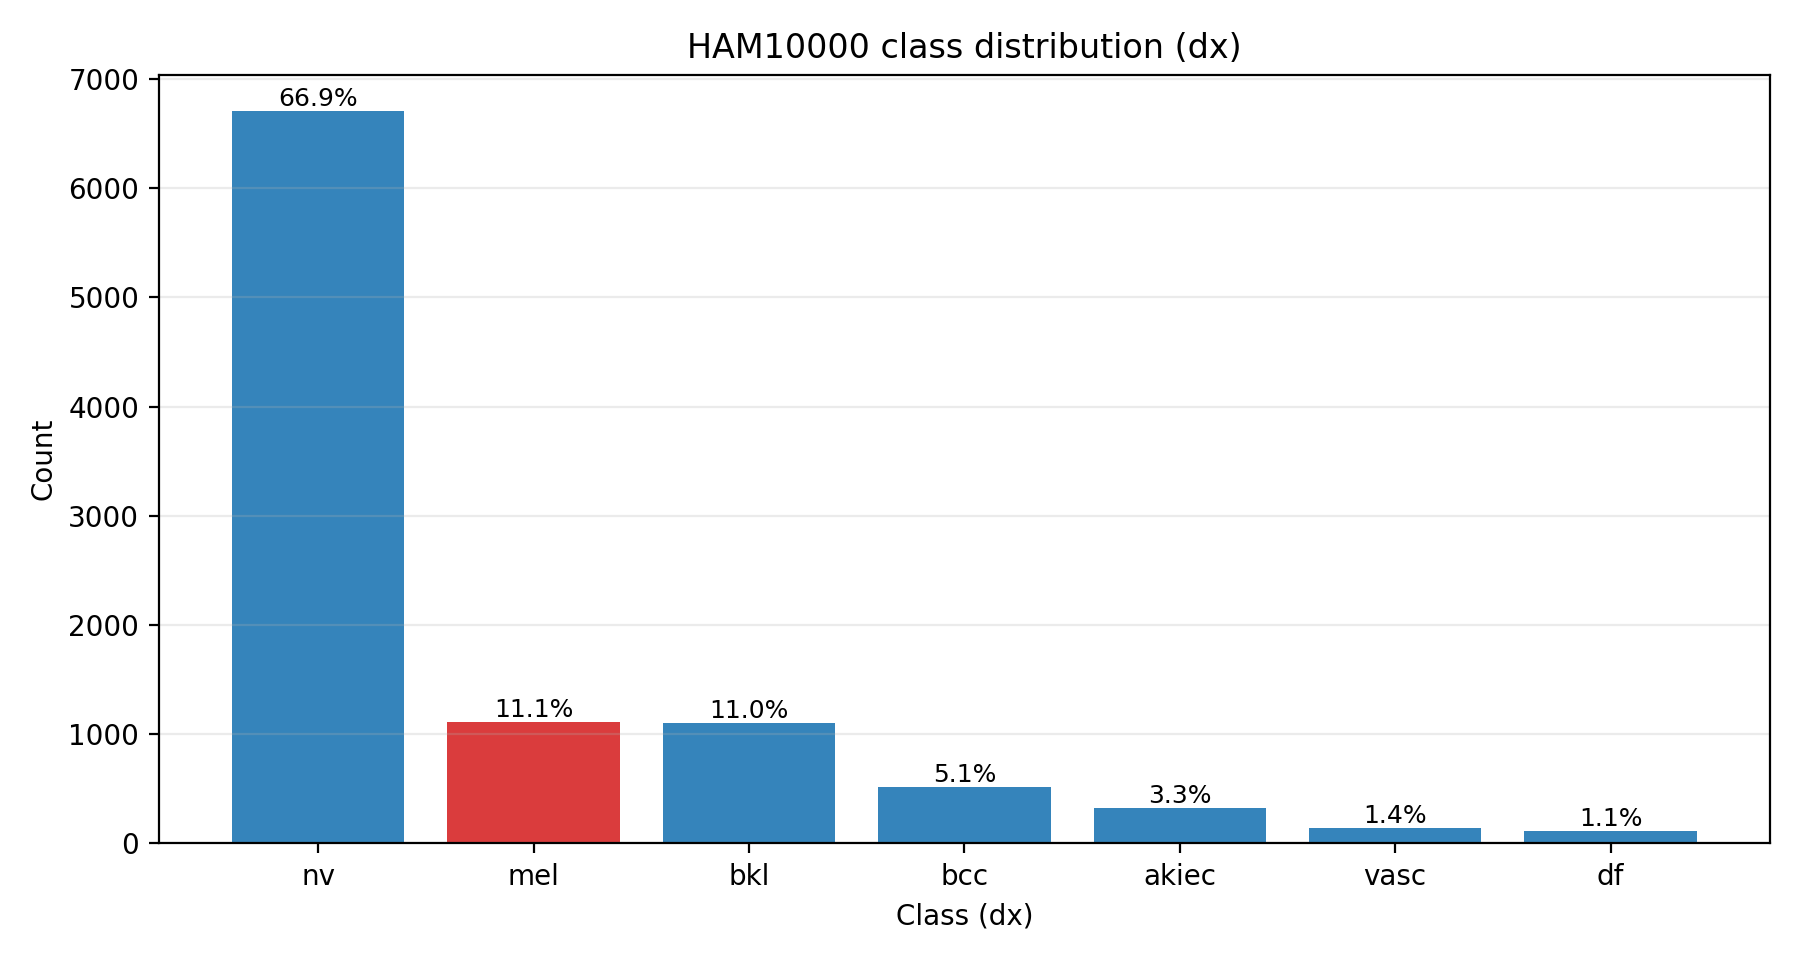
\includegraphics[width=0.95\columnwidth]{figures/class_distribution.png}
  \caption{HAM10000 class imbalance. The dominance of \texttt{nv} motivates macro-F1, per-class recall, and melanoma-focused evaluation in addition to accuracy.}
  \label{fig:classdist}
\end{figure}

\begin{table}[t]
  \centering
  \caption{Selected HAM10000 metadata descriptors used for dataset interpretation.}
  \label{tab:metadesc}
  \begin{tabular}{lr}
    \toprule
    Descriptor & Count \\
    \midrule
    \texttt{dx\_type = histo} & 5340 \\
    \texttt{dx\_type = follow\_up} & 3704 \\
    \texttt{dx\_type = consensus} & 902 \\
    \texttt{dx\_type = confocal} & 69 \\
    \texttt{dataset = vidir\_molemax} & 3954 \\
    \texttt{dataset = vidir\_modern} & 3363 \\
    \texttt{dataset = rosendahl} & 2259 \\
    \texttt{dataset = vienna\_dias} & 439 \\
    \bottomrule
  \end{tabular}
\end{table}

\begin{figure}[t]
  \centering
  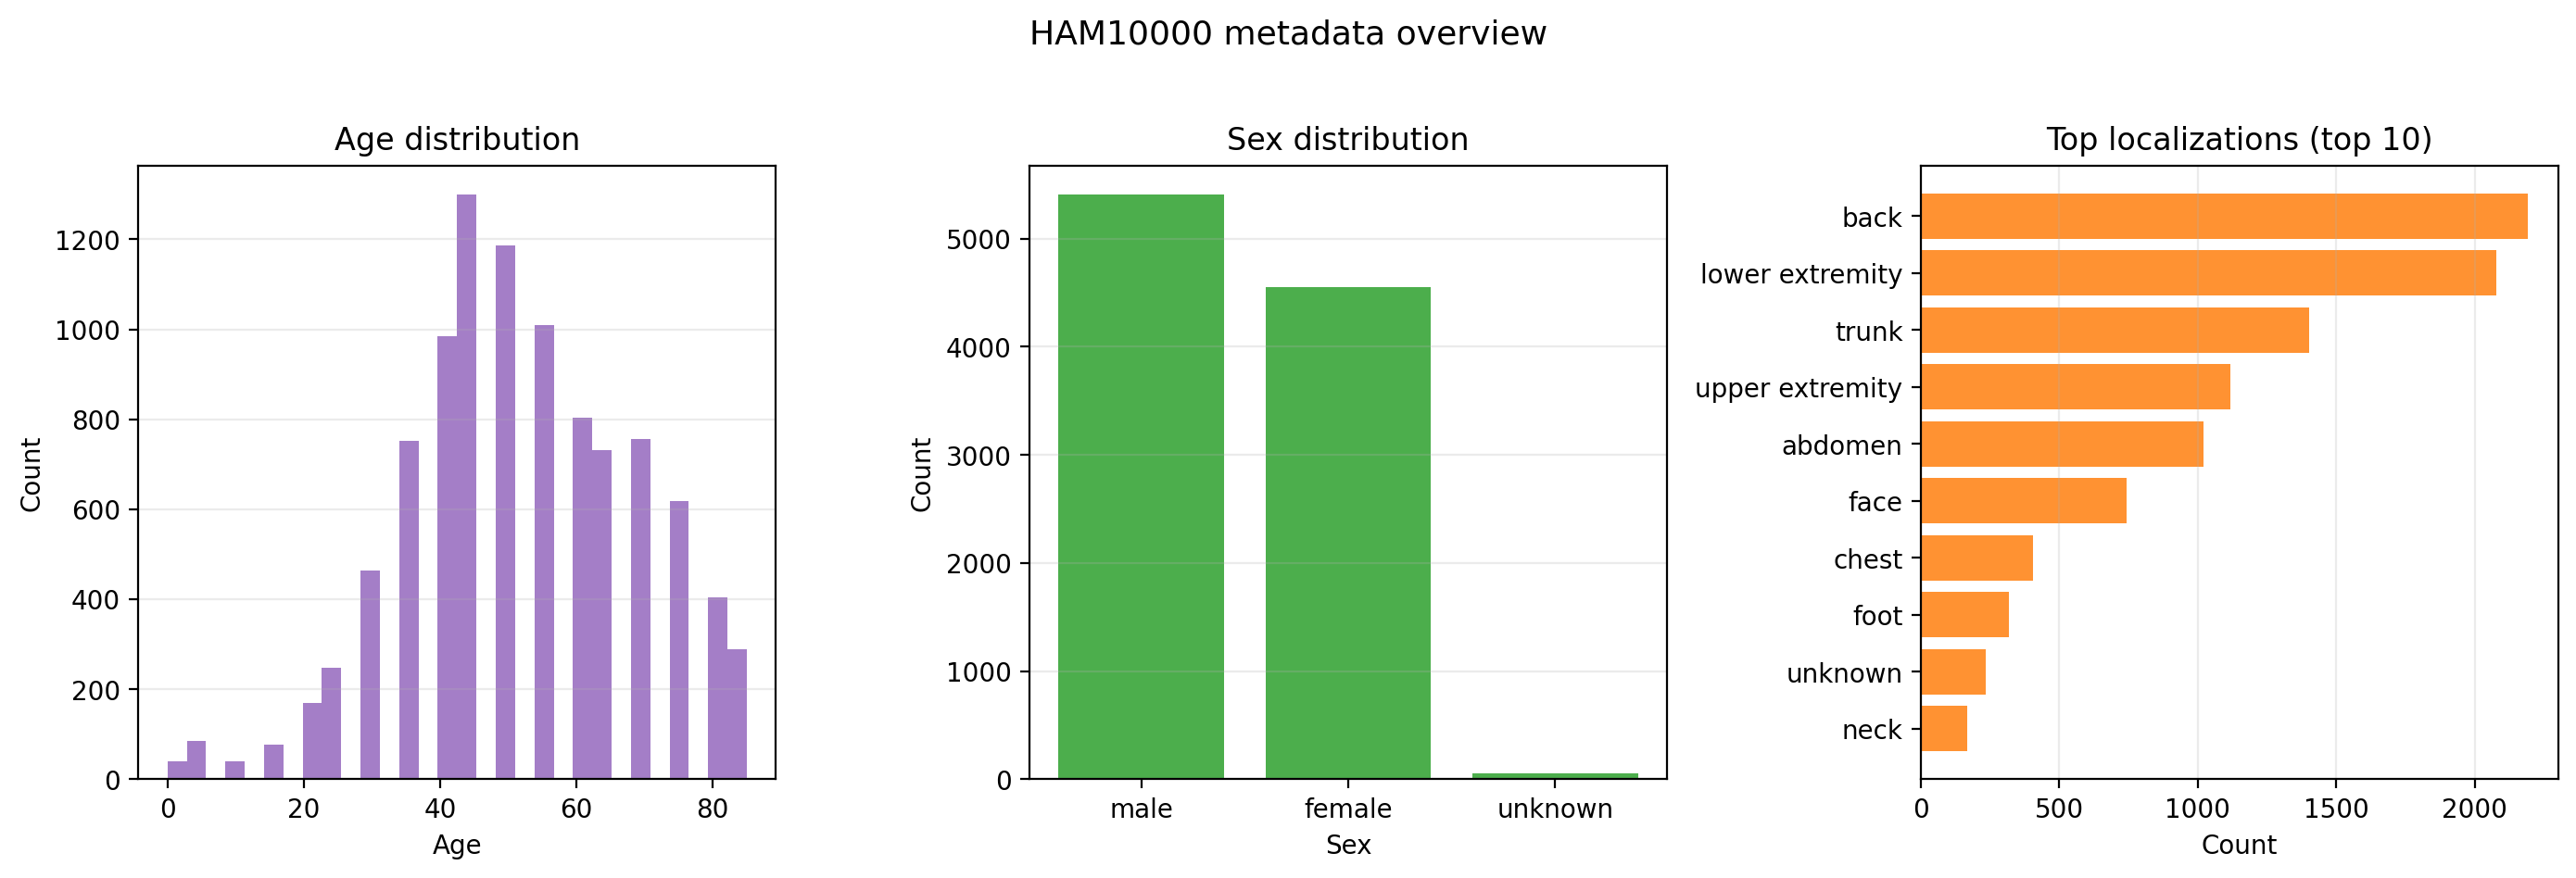
\includegraphics[width=0.98\columnwidth]{figures/metadata_stats.png}
  \caption{Metadata overview from the HAM10000 CSV. Age, sex, and localization distributions help contextualize subgroup and bias analysis.}
  \label{fig:metadata}
\end{figure}

\begin{figure}[t]
  \centering
  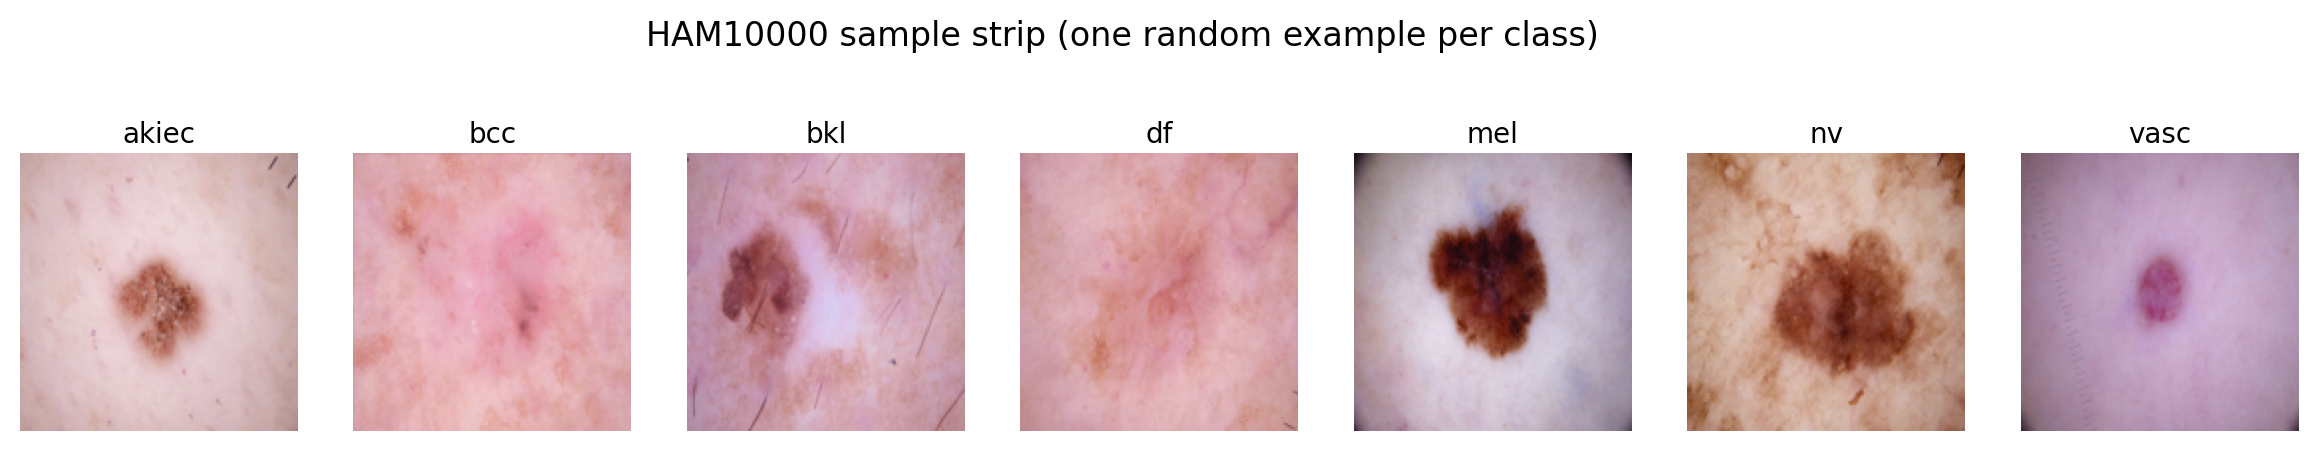
\includegraphics[width=0.98\columnwidth]{figures/samples_strip.png}
  \caption{Representative sample strip from the seven diagnostic categories. Visual overlap across classes helps explain difficult melanoma versus benign-lesion confusions.}
  \label{fig:samples}
\end{figure}

Table~\ref{tab:metadesc} and Fig.~\ref{fig:metadata} make the dataset heterogeneity concrete. Different diagnosis types imply different label provenance, while the source subsets indicate that HAM10000 is not a single-camera, single-clinic collection. Fig.~\ref{fig:samples} shows why some classes remain difficult even with a strong CNN backbone: color, texture, and lesion shape overlap across melanoma and benign pigmented lesions.

\section{Method}
\subsection{Classifier and Training}
The base classifier is EfficientNet with an ImageNet-pretrained backbone and a dropout-plus-linear classification head \cite{tan2019efficientnet}. Images are resized to a fixed square resolution, normalized with ImageNet statistics, and augmented with flips, rotations, color jitter, and optional random resized crop. Training uses AdamW \cite{loshchilov2019adamw} with mixed precision when CUDA is available.

Given logits $z$ over $K=7$ classes, the predicted probability for class $k$ is
\begin{equation}
p_k = \frac{\exp(z_k)}{\sum_{j=1}^{K}\exp(z_j)}.
\end{equation}

The best checkpoint is selected using one validation metric at a time, such as validation macro-F1, validation accuracy, or validation melanoma recall. This choice is part of the experimental design rather than only an implementation detail.

\subsection{Imbalance Handling and Screening View}
The project evaluates several lightweight imbalance interventions:
\begin{itemize}
\item class-weighted cross-entropy,
\item weighted random sampling,
\item melanoma-specific upweighting,
\item optional focal loss \cite{lin2017focal},
\item a small cVAE-based synthetic augmentation ablation.
\end{itemize}

For class-weighted cross-entropy,
\begin{equation}
\mathcal{L}_{\mathrm{WCE}} = -w_y \log(p_y),
\end{equation}
where $w_y$ is larger for minority classes and can be increased further for melanoma.

Beyond top-1 multiclass prediction, melanoma is also treated as a one-vs-rest screening target using the score $s(x)=P(\texttt{mel}\mid x)$. A threshold $t$ defines a melanoma alarm:
\begin{equation}
\hat{y}_{\mathrm{mel}}(x;t) = \mathbf{1}[s(x)\ge t].
\end{equation}
This makes the precision-recall trade-off explicit instead of hiding it inside a single top-1 label.

The broader report also discusses alternatives such as class-balanced losses based on effective sample count \cite{cui2019classbalanced}. I keep that point here only to show that the imbalance problem was explored beyond one fixed loss.

\subsection{Post-hoc Diagnostics}
To extend evaluation without retraining, I analyze saved test probabilities from completed runs. First, confidence calibration is summarized with a reliability diagram, confidence histogram, expected calibration error (ECE), and Brier score. With confidence bins $S_b$,
\begin{equation}
\mathrm{ECE} = \sum_{b=1}^{B}\frac{|S_b|}{n}\left|\mathrm{acc}(S_b)-\mathrm{conf}(S_b)\right|.
\end{equation}

Second, the shared test split is joined with HAM10000 metadata using \texttt{image\_id}, and melanoma recall is summarized across sex and age buckets. Metadata is used only for analysis, not as a model input.

\subsection{Evaluation Metrics}
Because HAM10000 is imbalanced, I report multiple metrics rather than accuracy alone. Accuracy summarizes global correctness, but macro-F1 gives all classes equal weight and is therefore more informative for minority classes. Per-class recall is especially important because melanoma recall corresponds to sensitivity for the most clinically concerning class. Together, these metrics distinguish a model that is generally strong from one that is specifically safer for melanoma detection.

\section{Experimental Setup}
All experiments use the same lesion-wise split and report test accuracy, macro-F1, per-class recall, confusion matrices, and melanoma threshold curves. The main tracked runs are baseline EfficientNet-B0, EfficientNet-B0 with sampling, EfficientNet-B0 with melanoma upweighting, EfficientNet-B0 with synthetic augmentation, and several EfficientNet-B2 variants with different resolutions and checkpoint selection policies.

The protocol is designed so that differences in behavior can be attributed mainly to imbalance handling, backbone capacity, input resolution, and checkpoint selection metric. This is important because in medical imaging a small metric change can otherwise be difficult to interpret if several training choices move simultaneously.

Table~\ref{tab:mainruns} shows the representative runs. The main comparison is intentionally built around an accuracy-focused model versus sensitivity-focused settings.

\begin{table}[t]
  \centering
  \caption{Representative test results on the fixed lesion-wise split.}
  \label{tab:mainruns}
  \begin{tabular}{lccc}
    \toprule
    Run & Acc & Macro-F1 & Mel recall \\
    \midrule
    Baseline (EffNet-B0) & 0.7637 & 0.6650 & 0.7581 \\
    Sampler (EffNet-B0) & 0.8006 & 0.6756 & 0.7016 \\
    Synth. aug. (EffNet-B0) & 0.7926 & 0.6979 & 0.6694 \\
    EffNet-B2 @224 mel-select & 0.7697 & 0.6958 & 0.7823 \\
    EffNet-B2 @260 acc-select & \textbf{0.8614} & \textbf{0.7386} & 0.5403 \\
    EffNet-B2 @260 mel-sampler & 0.5374 & 0.5666 & \textbf{0.8548} \\
    \bottomrule
  \end{tabular}
\end{table}

\section{Results and Analysis}
\subsection{Accuracy-Focused Versus Sensitivity-First}
The strongest multiclass classifier is EfficientNet-B2 at 260px selected by validation accuracy. It achieves 0.8614 test accuracy and 0.7386 macro-F1, but its top-1 melanoma recall is only 0.5403. In contrast, the sensitivity-first 260px model raises melanoma recall to 0.8548, but overall accuracy drops to 0.5374. This confirms that high overall accuracy can coexist with weak melanoma sensitivity on an imbalanced dataset.

\begin{figure}[t]
  \centering
  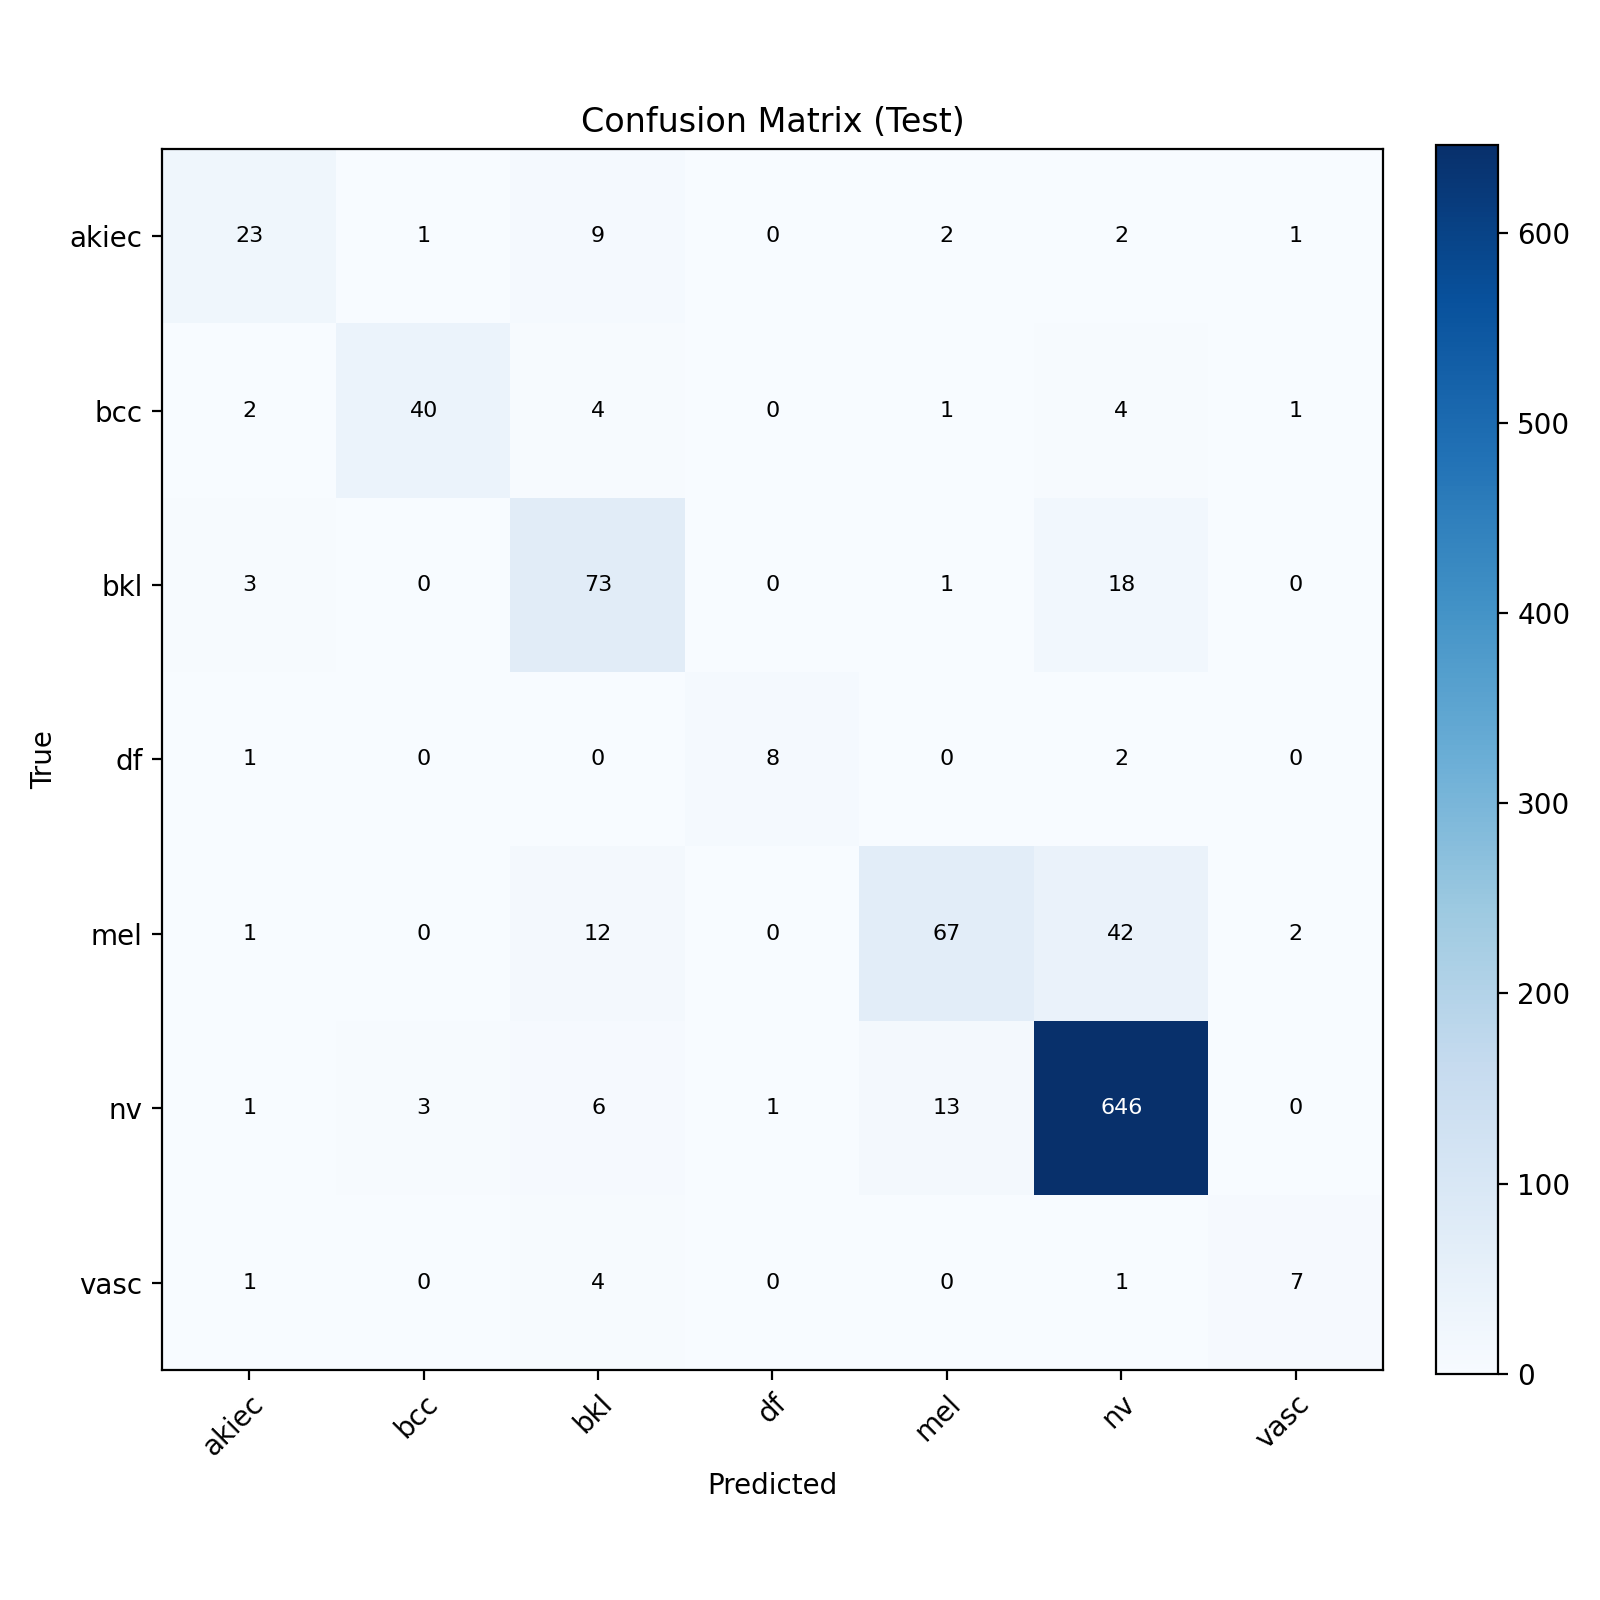
\includegraphics[width=0.80\columnwidth]{figures/confusion_matrix_effnetb2_260_acc.png}
  \caption{Confusion matrix of the accuracy-focused EfficientNet-B2@260 run. Strong \texttt{nv} performance drives overall accuracy, but many melanoma samples are still confused with pigmented benign classes.}
  \label{fig:cmacc}
\end{figure}

The confusion matrix in Fig.~\ref{fig:cmacc} shows why this happens. The model is very strong on \texttt{nv}, which dominates the test set, while melanoma is still frequently confused with \texttt{nv} and \texttt{bkl}. This is exactly the kind of failure pattern that can be obscured by accuracy alone.

\begin{figure}[t]
  \centering
  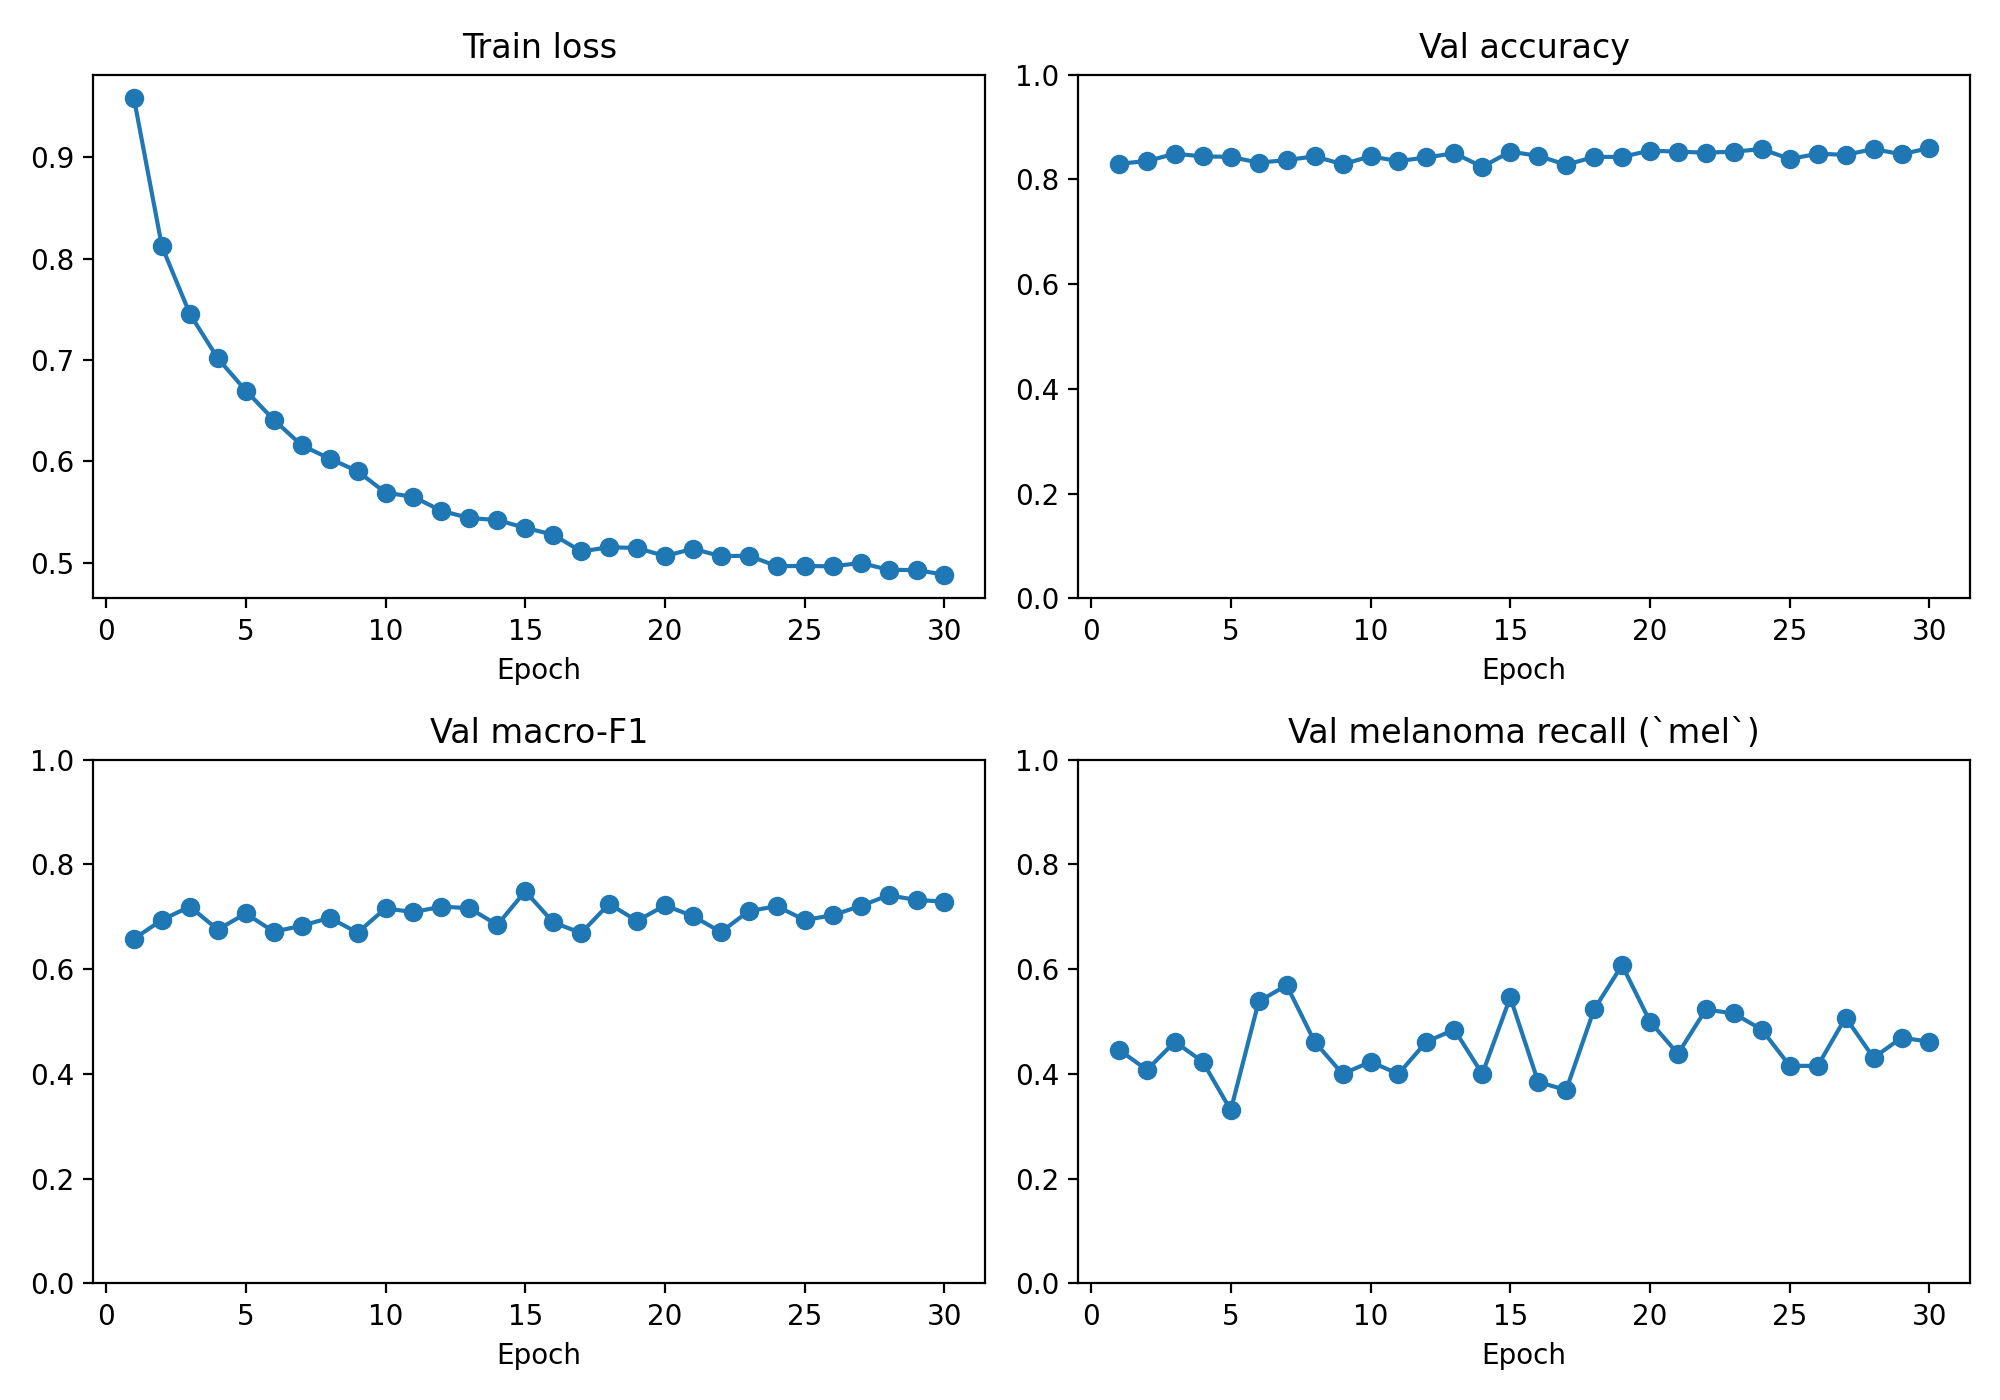
\includegraphics[width=0.98\columnwidth]{figures/training_curves_effnetb2_260_acc.png}
  \caption{Training dynamics for the accuracy-focused EfficientNet-B2@260 run. Validation accuracy improves steadily, while melanoma-specific behavior does not automatically track the same objective.}
  \label{fig:traincurve}
\end{figure}

Table~\ref{tab:perclass} makes the trade-off clearer. The accuracy-focused run gets very high \texttt{nv} recall, while melanoma recall drops. The sensitivity-first model reverses that pattern and sacrifices \texttt{nv} heavily.

The training curves in Fig.~\ref{fig:traincurve} help explain the downstream trade-off. Once checkpoint selection is tied to validation accuracy, the optimization path naturally favors the dominant and easier classes. The behavior of the best accuracy-focused checkpoint is therefore consistent with the training objective rather than being a random artifact of one epoch.

\begin{table}[t]
  \centering
  \caption{Per-class recall for representative EfficientNet-B2 runs.}
  \label{tab:perclass}
  \begin{tabular}{lccc}
    \toprule
    Class & B2@260 acc & B2@224 mel & B2@260 sens \\
    \midrule
    \texttt{akiec} & 0.605 & 0.632 & 0.763 \\
    \texttt{bcc}   & 0.769 & 0.789 & 0.789 \\
    \texttt{bkl}   & 0.768 & 0.642 & 0.663 \\
    \texttt{df}    & 0.727 & 0.727 & 0.636 \\
    \texttt{mel}   & 0.540 & 0.782 & 0.855 \\
    \texttt{nv}    & 0.964 & 0.794 & 0.421 \\
    \texttt{vasc}  & 0.538 & 0.692 & 0.846 \\
    \bottomrule
  \end{tabular}
\end{table}

\subsection{Threshold-Based Melanoma Screening}
Thresholding $P(\texttt{mel})$ turns the multiclass classifier into a screening-oriented detector. For the melanoma-aware EfficientNet-B2 at 224px, the selected operating point satisfying recall $\ge 0.85$ reaches precision $\approx 0.322$ and recall $\approx 0.855$. The accuracy-focused 260px model can also achieve very high melanoma recall by lowering the threshold aggressively, but its precision becomes much worse.

\begin{figure}[t]
  \centering
  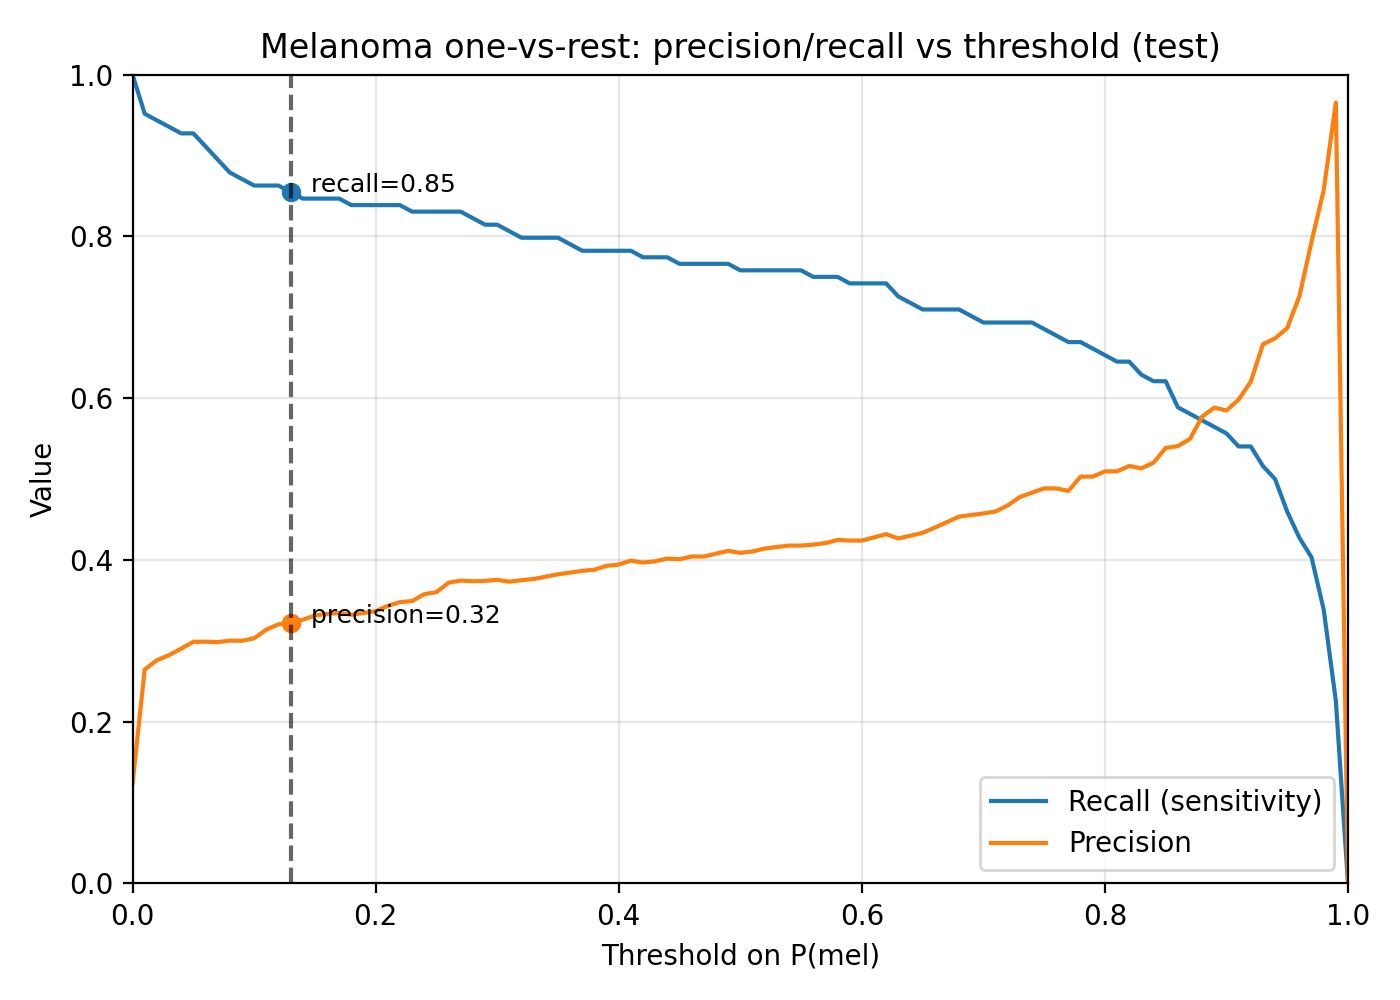
\includegraphics[width=0.98\columnwidth]{figures/mel_threshold_curve_effnetb2.png}
  \caption{Threshold-based melanoma screening. Lower thresholds increase recall but cause many more false positives.}
  \label{fig:threshold}
\end{figure}

This is the practical takeaway from Fig.~\ref{fig:threshold}: the same backbone can serve different decision styles, but screening-oriented operation must be presented with precision-recall trade-offs, not only top-1 labels.

\begin{figure}[t]
  \centering
  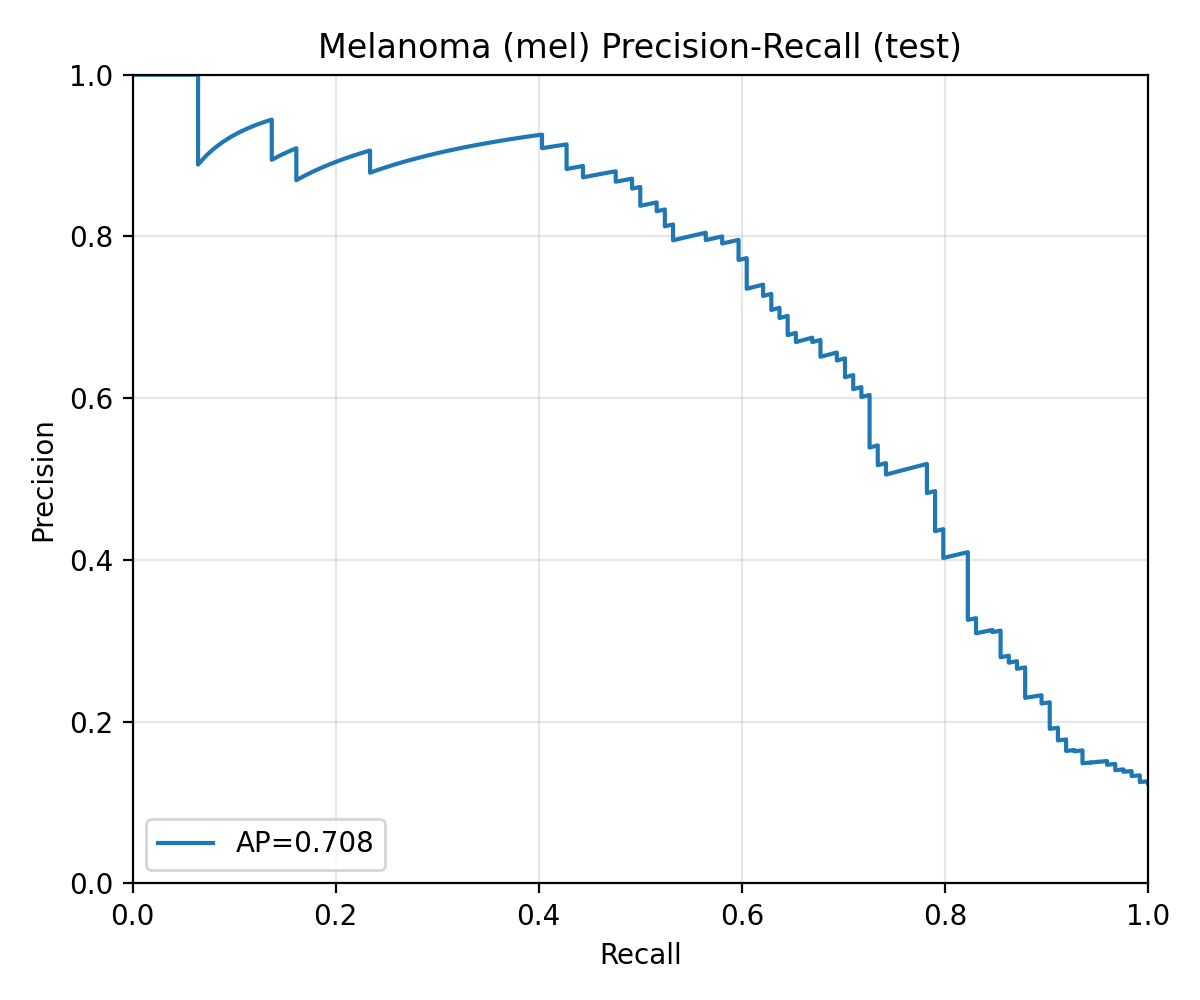
\includegraphics[width=0.98\columnwidth]{figures/mel_pr_curve_effnetb2_260_acc.png}
  \caption{Melanoma precision-recall curve for the accuracy-focused model. The curve reinforces that high melanoma recall is achievable only with a substantial precision cost.}
  \label{fig:melpr}
\end{figure}

\begin{table}[t]
  \centering
  \caption{Selected melanoma screening operating points.}
  \label{tab:thresholdops}
  \begin{tabular}{lcccc}
    \toprule
    Model & Recall target & $t$ & Prec. & Rec. \\
    \midrule
    B2@224 mel-select & $\ge 0.85$ & 0.13 & 0.322 & 0.855 \\
    B2@224 mel-select & $\ge 0.90$ & 0.06 & 0.299 & 0.911 \\
    B2@260 acc-select & $\ge 0.85$ & 0.01 & 0.133 & 0.992 \\
    B2@260 mel-sampler & $\ge 0.85$ & 0.34 & 0.222 & 0.855 \\
    \bottomrule
  \end{tabular}
\end{table}

Table~\ref{tab:thresholdops} and Fig.~\ref{fig:melpr} show why the melanoma-aware 224px model is the better screening candidate. It provides a more favorable precision-recall trade-off than the accuracy-focused model, which only reaches very high recall at extremely low thresholds and therefore produces many more false positives.

\subsection{Confidence Reliability}
The added post-hoc analysis shows that the accuracy-focused model is useful but not perfectly calibrated. Its mean top-1 confidence is 0.8735, slightly above its realized accuracy of 0.8614, with ECE 0.0484, Brier score 0.2211, and negative log-likelihood 0.5244.

\begin{figure}[t]
  \centering
  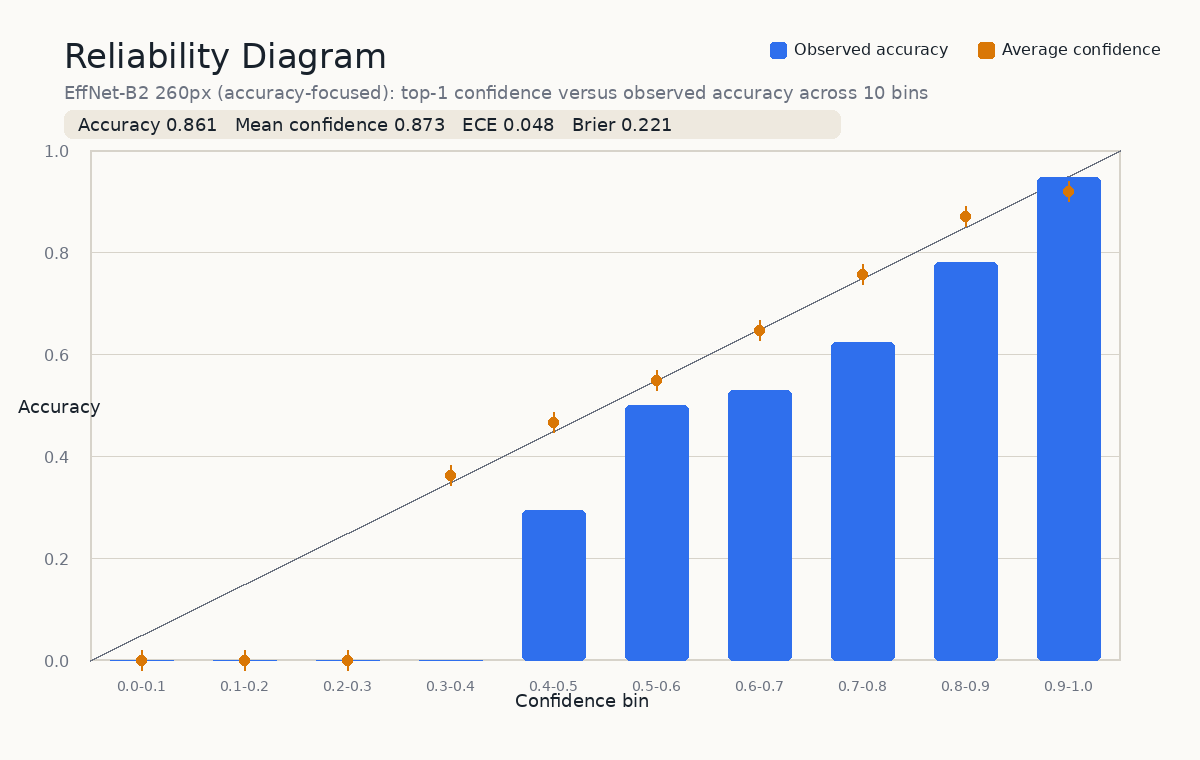
\includegraphics[width=0.98\columnwidth]{figures/reliability_effnetb2_260_acc.png}
  \caption{Reliability diagram for the accuracy-focused model. Confidence tracks accuracy reasonably well, but mild overconfidence remains in several bins.}
  \label{fig:reliability}
\end{figure}

Confidence quality is therefore not catastrophic, but it is not decision-ready either. This matters because any thresholding policy or user-facing probability display implicitly assumes that model confidence has some operational meaning.

\begin{figure}[t]
  \centering
  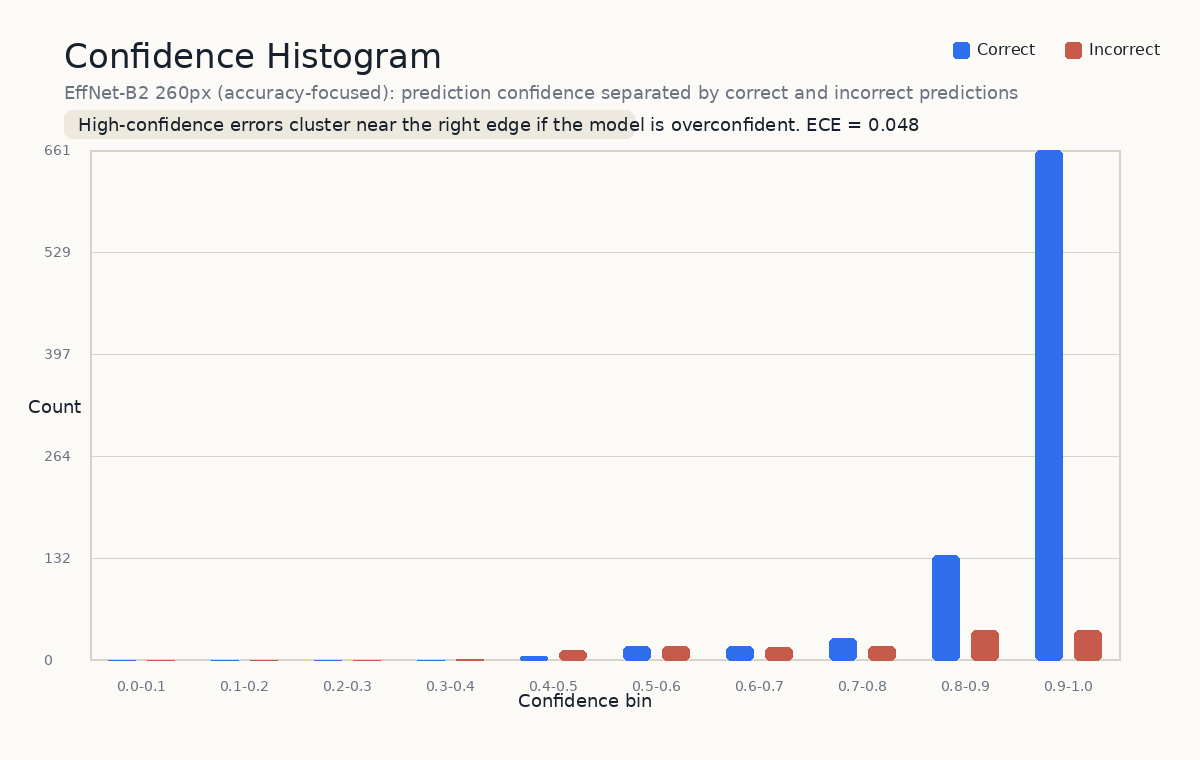
\includegraphics[width=0.98\columnwidth]{figures/confidence_hist_effnetb2_260_acc.png}
  \caption{Confidence histogram for the accuracy-focused model. Some incorrect predictions still occur in the high-confidence region, indicating overconfident errors.}
  \label{fig:confhist}
\end{figure}

The confidence histogram in Fig.~\ref{fig:confhist} is useful because it reveals that some wrong predictions are made with strong confidence. That kind of error is more concerning than a low-confidence mistake, especially in an interface that exposes predicted probabilities to users.

\subsection{Metadata Subgroup Analysis}
The subgroup analysis shows that melanoma recall is not uniform across the shared test split. The accuracy-focused model is weakest for female patients and for the oldest age bucket, while the sensitivity-first model improves melanoma recall across all observed subgroups but with a much higher false-positive burden.

\begin{figure}[t]
  \centering
  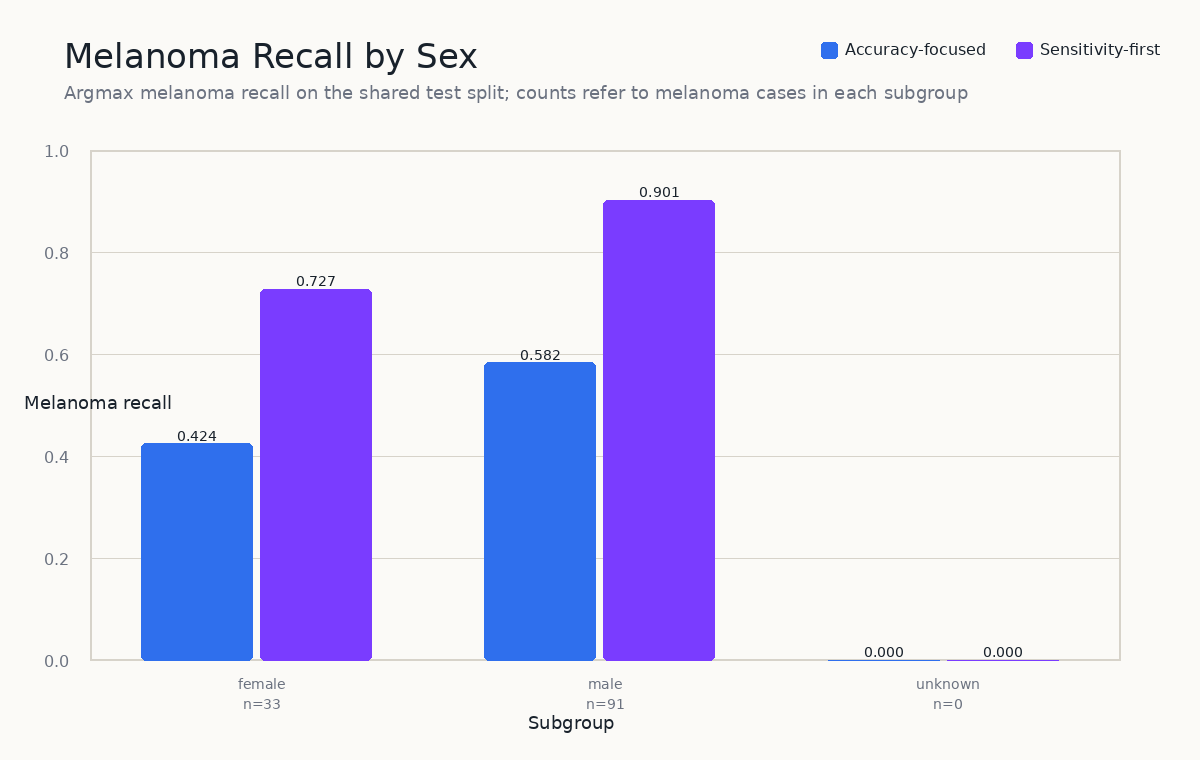
\includegraphics[width=0.98\columnwidth]{figures/mel_recall_by_sex_compare.png}
  \caption{Melanoma recall by sex. The sensitivity-first model improves recall for both male and female patients, but the accuracy-focused model is noticeably weaker on the female subgroup.}
  \label{fig:sexgroup}
\end{figure}

\begin{figure}[t]
  \centering
  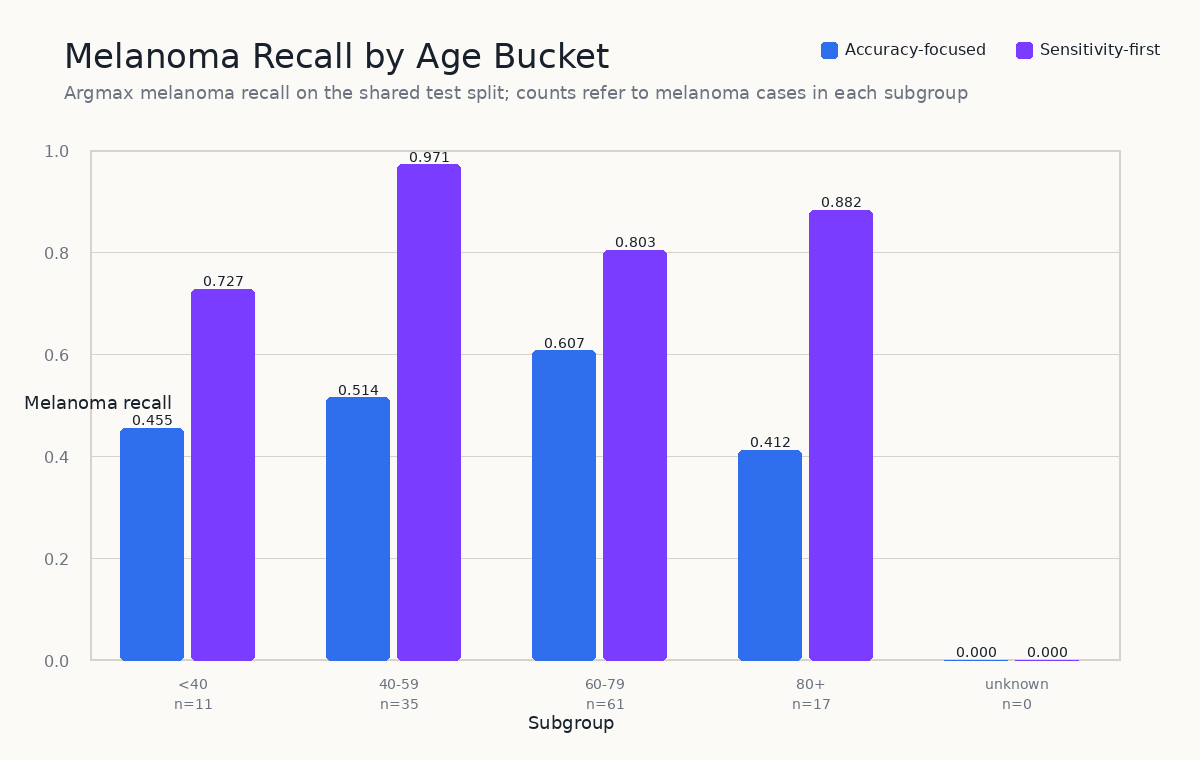
\includegraphics[width=0.98\columnwidth]{figures/mel_recall_by_age_compare.png}
  \caption{Melanoma recall by age bucket. The sensitivity-first model improves recall across all age groups with melanoma cases, while the accuracy-focused model is weakest in the \texttt{80+} bucket.}
  \label{fig:agegroup}
\end{figure}

\begin{table}[t]
  \centering
  \caption{Melanoma recall by subgroup on the shared test split.}
  \label{tab:subgroups}
  \begin{tabular}{lccc}
    \toprule
    Subgroup & Acc.-focused & Sens.-first & Mel cases \\
    \midrule
    Female & 0.424 & 0.727 & 33 \\
    Male & 0.582 & 0.901 & 91 \\
    $<40$ & 0.455 & 0.727 & 11 \\
    40--59 & 0.514 & 0.971 & 35 \\
    60--79 & 0.607 & 0.803 & 61 \\
    80+ & 0.412 & 0.882 & 17 \\
    \bottomrule
  \end{tabular}
\end{table}

Figures~\ref{fig:sexgroup} and \ref{fig:agegroup} make the pattern visually clear: the accuracy-focused model is not uniformly strong across subgroups, and the aggregate melanoma recall can hide uneven behavior across simple patient groups.

\subsection{Practical Interpretation}
Two patterns summarize the main findings. First, melanoma is most often confused with \texttt{nv} and \texttt{bkl}; this is why the accuracy-focused model can remain strong overall while still missing many melanoma cases. Second, explicitly optimizing for melanoma recall shifts many benign nevi toward melanoma, which makes the sensitivity-first classifier hard to use as a general multiclass predictor. A strong submission story is therefore to pair an accuracy-focused model with melanoma-specific threshold analysis, and then use calibration and subgroup diagnostics to show where caution is still necessary.

Another practical lesson is that model selection and operating-point selection should be treated separately. Validation-accuracy selection produces the strongest general classifier, but the best screening threshold is better obtained from a melanoma-aware model whose probability distribution is more favorable for precision-recall control. In other words, the project does not support a single universal ``best'' checkpoint; it supports different recommended operating modes for different goals.

\subsection{Training Behavior and Error Sources}
The longer project report also shows that the accuracy-focused EfficientNet-B2@260 run has stable validation behavior and a relatively clean separation between optimization for global accuracy and optimization for melanoma recall. In practical terms, the model selected by validation accuracy behaves exactly as expected: it becomes very good at the dominant \texttt{nv} class and improves macro-F1, but it does not naturally converge to a melanoma-sensitive operating point. This is useful to state explicitly because it shows that the low top-1 melanoma recall is not an implementation accident; it is a consequence of the selected objective.

Weighted sampling, melanoma upweighting, and synthetic augmentation all alter the effective training distribution, but they redistribute performance across classes rather than improving every target at once. The main conflict is between preserving very strong \texttt{nv} recall and reducing false negatives on melanoma. From a course-submission perspective, this leads to a concrete recommendation: use EfficientNet-B2@260 as the headline multiclass model, and use the melanoma-aware EfficientNet-B2@224 configuration for threshold-based screening discussion.

\section{Interpretability and Demo}
The full project also includes Grad-CAM-based interpretability and a Streamlit demo application. These components are not the main scientific contribution of the paper, but they strengthen the final course deliverable by making model behavior easier to inspect, which is also how they are presented in the longer report.

Grad-CAM overlays help check whether the model attends to lesion regions rather than obviously irrelevant background cues \cite{selvaraju2017gradcam}. In presentation settings, this is useful for showing both plausible successes and clinically meaningful failure cases, such as missed melanomas despite lesion-focused attention.

\begin{figure}[t]
  \centering
  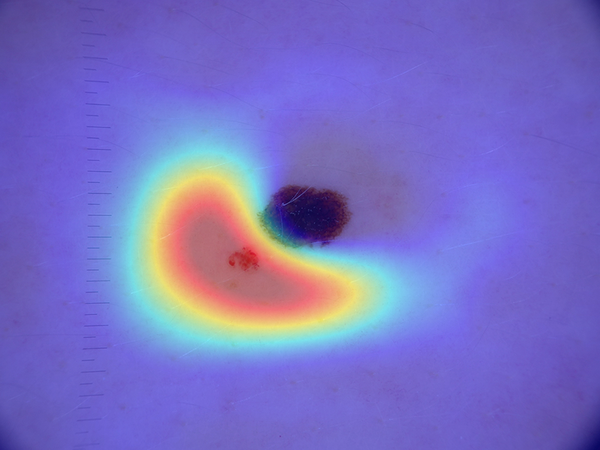
\includegraphics[width=0.92\columnwidth]{figures/ISIC_0025964_overlay.png}
  \caption{Representative Grad-CAM overlay. In the full report, Grad-CAM is used as a qualitative sanity check for whether model attention overlaps the lesion region.}
  \label{fig:gradcam}
\end{figure}

In the longer project report, one illustrative case is a melanoma image that the baseline model predicts incorrectly while still producing a focused attention map. That kind of example matters because it shows that explanation alone does not guarantee correctness; sensitivity-oriented evaluation is still necessary.

\begin{figure}[t]
  \centering
  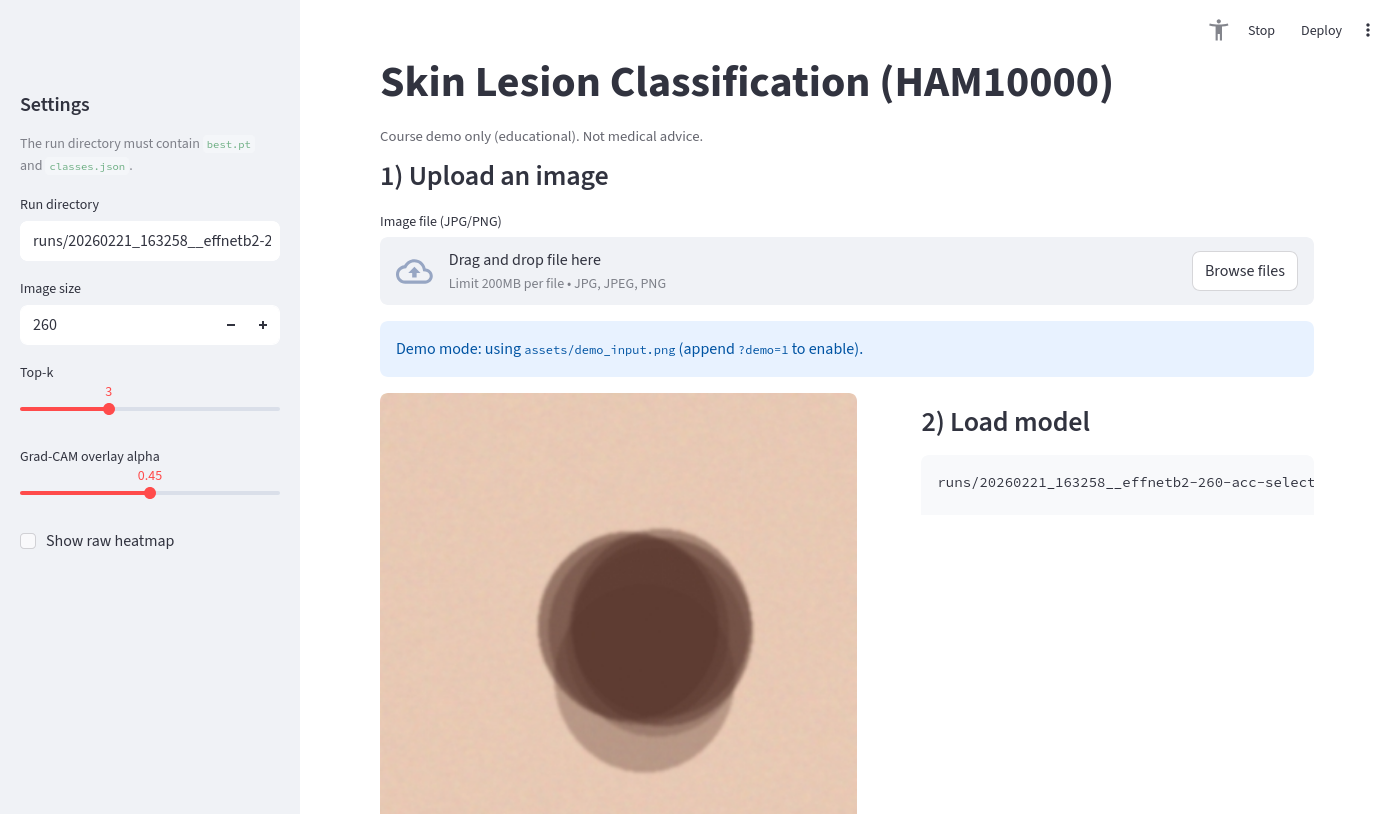
\includegraphics[width=0.98\columnwidth]{figures/streamlit_demo.png}
  \caption{Streamlit demo interface for image upload, class probabilities, and visual explanation. This supports a practical end-to-end demonstration of the system.}
  \label{fig:demo}
\end{figure}

The Streamlit app further turns the trained model into a usable interface with image upload, top-$k$ predictions, and Grad-CAM visualization. For a final project, this matters because it demonstrates that the model can be packaged into a real workflow rather than remaining only as offline experiments \cite{streamlitdocs}.

\section{Reproducibility, Ethics, and Conclusion}
The repository includes tracked experiment configurations, saved run metadata, result plots, and a demo application, allowing the main comparisons and figures to be regenerated from code. Even so, the system should not be interpreted as clinical decision support: HAM10000 is limited, external validation is absent, and some subgroup counts are small.

This work should therefore be read as an educational prototype for medical-AI evaluation. On a single lesion-wise split, the accuracy-focused model gives the best multiclass performance, the sensitivity-first model gives the strongest top-1 melanoma recall, and the added post-hoc diagnostics show that calibration and subgroup consistency impose additional constraints beyond either objective alone. Together, these results demonstrate a complete deep-learning workflow for dermatoscopic image classification while leaving external validation and explicit calibration correction for future work.

\bibliographystyle{IEEEtran}
\bibliography{references}

\end{document}
